\chapter{Towards a model}\label{chapter:model}
In this chapter we derive a model for an iptables-enabled device using SEFL.
We start with a simple one, and increase its complexity and the amount of
details as we gradually introduce features that allow us to express more and
more complex iptables rules.  We sum up with an overview of the limitations
encountered along the way.


\section{Making the first steps}\label{sec:first-steps}

Building a SEFL model which can then be verified by SymNet is as simple as
providing two Map data structures, as discussed in
\labelindexref{Section}{sec:symnet-sefl}:
\begin{enumerate}[a)]
  \item the first one, from \emph{source} ports to \emph{destination} ports; it
    implicitly defines a directed graph which is our formal way of defining
    networks.
  \item the other one, from \emph{ports} (i.e. nodes in this graph) to SEFL
    instructions; this one captures the actual behaviour of each network
    element.
\end{enumerate}

The goal of this chapter is to show how we provide these Maps starting from a
deployment of iptables rules, in such a way that once fed into SymNet, the
verified behaviour is that of an iptables-enabled device.  To do so, in this
section we start by describing the high-level idea of our model as well as the
underlying algorithms that we use.

\bigskip

To ease the bootstrapping of our modelling process, we notice that packet
processing in netfilter is built around the routing decision.  To be more
precise, in \labelindexref{Figure}{fig:iptables-organization} from the previous
chapter there are three points in the processing stack where the routing table
is consulted.  Moreover, a routing decision was the only feature of the simple
router model we introduced in \labelindexref{Section}{sub-sec:building-models}.
Well-known software engineering practices tell us that we should reuse existing
functionality as long as it makes sense to do so.  In our scenario, it does.

Thus, in the first iteration towards our end goal of reaching an iptables model
from a router model we separate the only routing decision featured in
\labelindexref{Figure}{fig:router-model} into three different routing
decisions, as shown in \labelindexref{Figure}{fig:iptables-1}.

\begin{figure}[h]
  \centering
  \captionsetup{justification=centering}
  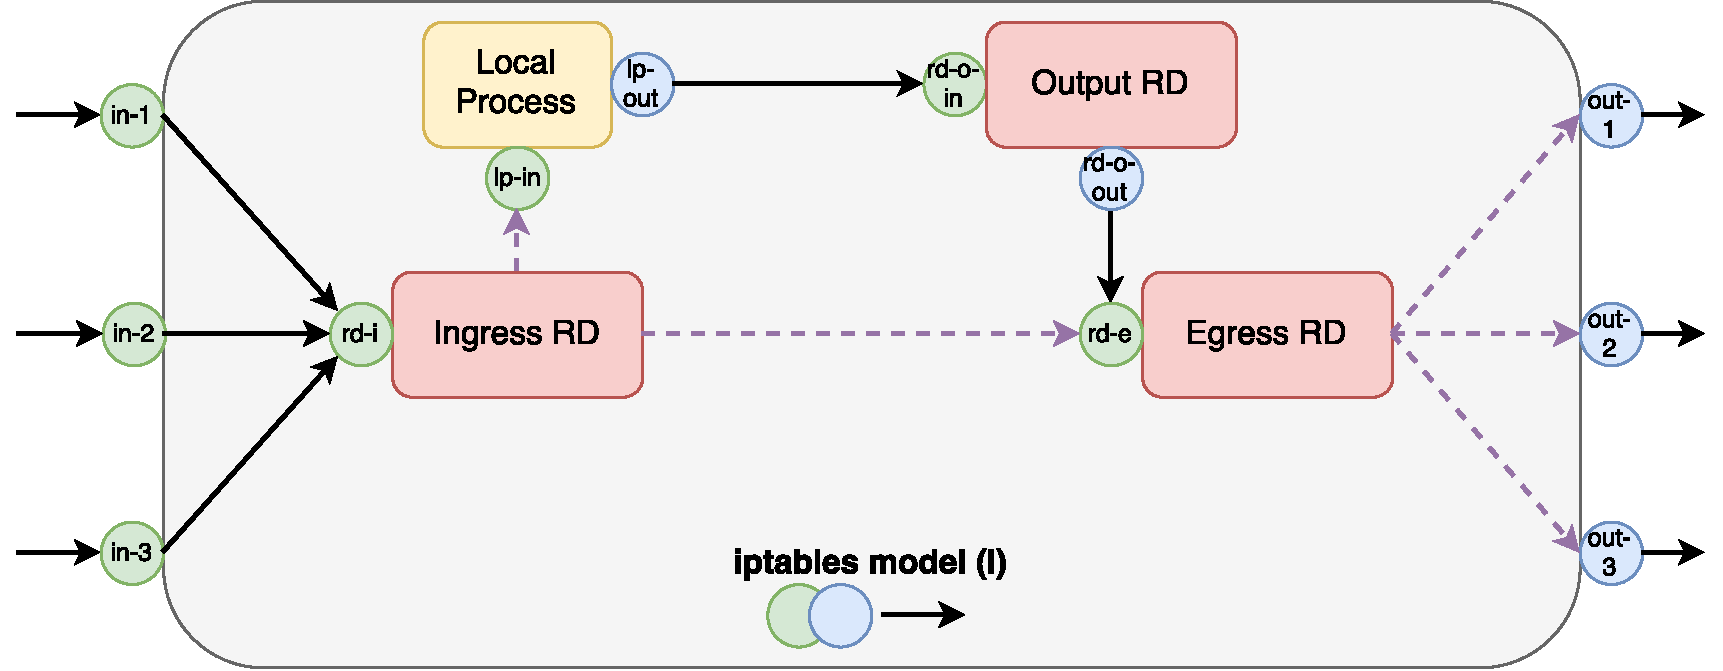
\includegraphics[scale=0.5]{assets/img/iptables-1}
  \caption[iptables model (I): Separated routing decisions.]{iptables model
  (I): Separated routing decisions.  Straight arrows correspond to directed
  edges in our network model, while dotted-arrows correspond to possible
  \emph{Forward} instructions directing traffic on those paths. Note that it is
  important to assign unique port names because there are no name scopes;
  implementation-wise, this is achieved by prefixing the \emph{role} of the
  port (e.g.  \emph{in}, \emph{out}) by the unique name of the \emph{virtual
  device} it belongs to.}
  \label{fig:iptables-1}
\end{figure}

Note that we \emph{specialized} each one of the three new routing decisions:
\begin{itemize}
  \item \textbf{ingress} routing decision: for traffic that \textbf{enters}
    this device
  \item \textbf{egress} routing decision: for traffic that \textbf{exits} this
    device
  \item \textbf{output} (sometimes \emph{local}) routing decision: for traffic
    that is \textbf{generated by} this device
\end{itemize}

Another thing that might not be obvious at first is that the behaviour of two
out of three of them has changed.  It is easier to see this if we focus on the
one for locally generated packets.  We notice that its single output port is
connected to the input port of the \emph{egress} one, which means that all
packets that enter it will follow that path.  Thus, it does not capture the
usual routing decision behaviour which simply forwards packets to output ports
based on some logic (i.e. destination IP and routing table).  The same applies
to \emph{ingress} which only partitions packets based on whether they should be
delivered locally or not.  It turns out that this new behaviour is essential to
iptables, to enable matching against the output interface in the
FORWARD/POSTROUTING chains, or to allow redirecting traffic in nat/OUTPUT. It
is usually implemented by storing the decision (output port) instead of
forwarding packets based on it.

As simple as this step might be, it still corresponds to a valid iptables
configuration: the \emph{void} one.  This is a valuable remark because it
allows us to validate future, more complex versions of the model by comparing
their output when all chains/tables are empty to that of this
\emph{featureless} one (a form of \textbf{regression testing}).

\bigskip

To advance one more step in our attempt to reach a model of an iptables-enabled
device, let us observe the similarity between
\labelindexref{Figure}{fig:iptables-1} and
\labelindexref{Figure}{fig:iptables-organization} from
\labelindexref{Chapter}{chapter:background}.  It seems that all we need to do
in order to make them be truly alike is to add some \emph{virtual devices} to
model chain traversal. The resulting schema is shown in
\labelindexref{Figure}{fig:iptables-2}.

\begin{figure}[h]
  \centering
  \captionsetup{justification=centering}
  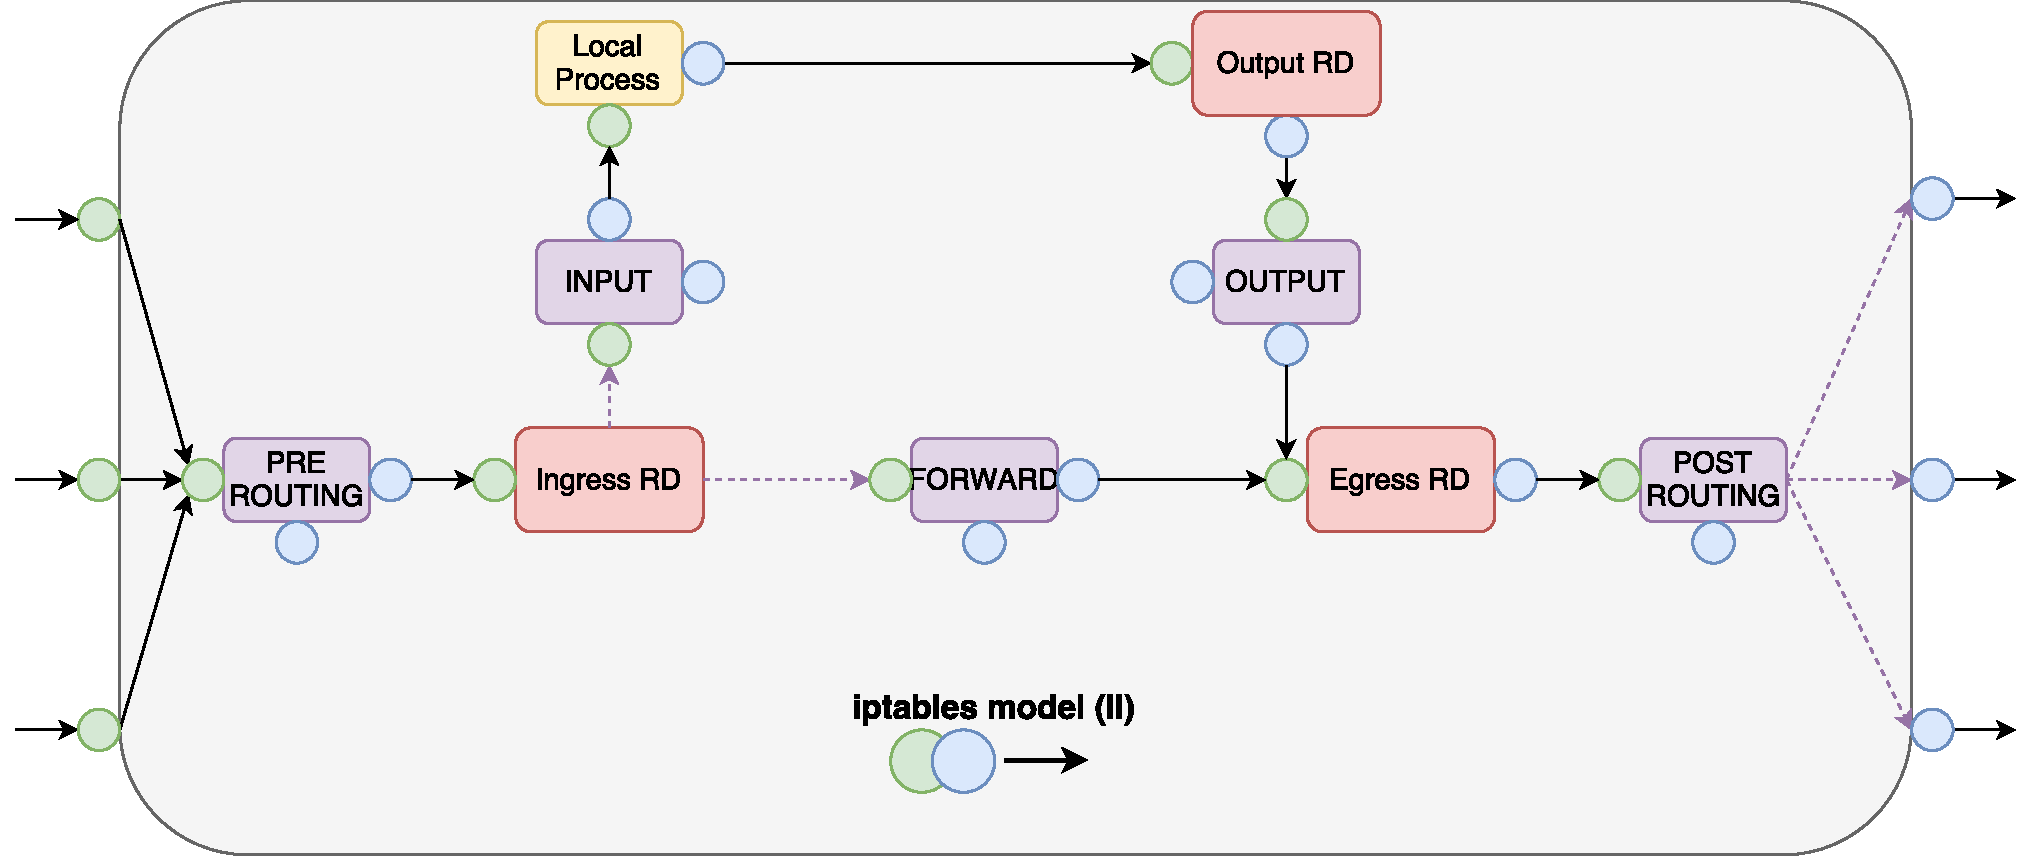
\includegraphics[scale=0.45]{assets/img/iptables-2}
  \caption[iptables model (II): Incorporated chain virtual devices.]{iptables
  model (II): Incorporated chain virtual devices.  The purple squares are
  Iptables Virtual Devices (IVDs) and they abstract chain traversal logic.}
  \label{fig:iptables-2}
\end{figure}

The new virtual devices are called \textbf{Iptables Virtual Devices}
(IVD)\abbrev{IVD}{Iptables Virtual Devices} and have the distinctive feature
that always have one input port and two output ports: an output port
corresponding to \emph{accepting} packets, whether modified or not, and another
one for \emph{dropping} packets, which is especially useful when modelling the
filter table.  In \labelindexref{Figure}{fig:iptables-2}, the former
corresponds to the output ports (blue circles) of IVDs (purple squares) which
are linked to the next virtual device in the processing stack.  On the other
hand, the \emph{dropping} ports are not connected to any other ports and have a
SEFL \hltexttt{Fail} instruction associated with them.

So what does this new augmented model buy us?  Firstly, as already mentioned,
it is closer (at least from a high-level perspective for now) to the internal
organization of iptables.  Secondly, it further separates the actual iptables
logic to be modelled on a per-chain basis.  In fact, this can be further
divided by acknowledging that each chain IVD, as it represented here, is a
sequence of concrete (per table) chain traversals; for instance, there are 3
tables that might define rules in the PREROUTING chain: raw, mangle, nat.
Therefore, we can improve our model by splitting each chain IVD as shown in
\labelindexref{Figure}{fig:iptables-2-composition}.

\begin{figure}[h]
  \centering
  \captionsetup{justification=centering}
  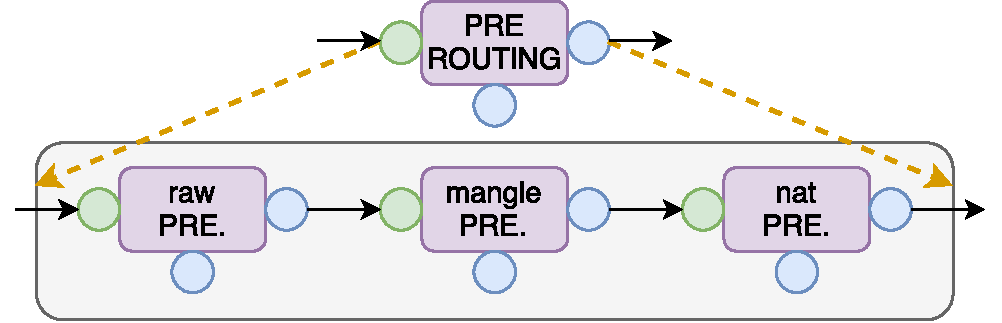
\includegraphics[scale=0.5]{assets/img/iptables-2-composition}
  \caption{Concrete (per-table) chains constitute a processing step.}
  \label{fig:iptables-2-composition}
\end{figure}

Thus, we claim that we reduced the problem of modelling an iptables-enabled
device to that of implementing (in SEFL) the traversal of a chain of rules.
\labelindexref{Algorithm}{algo:chain-traversal} captures the naive but
straightforward way of doing this.

\begin{algorithm}[H]
  \SetKwInOut{Inputs}{inputs}
  \SetKwInOut{Output}{output}
  \SetKwProg{TraverseChain}{TraverseChain}{}{}

  \TraverseChain{$(C, P)$}{
    \Inputs{A chain $C$ and a packet $P$}
    \Output{The target $T$ to jump to}

    \ForEach{rule $r \in$ C.rules}{
      \If{$m(p)$ is true $\forall m \in$ r.matches}{
        \textbf{return} $r.target$
      }
    }
    \textbf{return} $C.policy$
  }
  \caption[Traversing a chain.]{Traversing a chain. A chain aggregates a list
  of \emph{rules} and a \emph{default target} (i.e. policy). A rule contains a
  list of \emph{matches} and a \emph{target}.}
  \label{algo:chain-traversal}
\end{algorithm}

It is possible to express this algorithm in SEFL.  However, there are two
problems with it:
\begin{itemize}
  \item It \textbf{ignores} a couple of essential features in iptables (e.g.
    jumping to user-defined chains).  Thus,
    \labelindexref{Figure}{fig:iptables-2}, even though correct in terms of the
    abstractions it makes, hides a couple of rather involved functionality.
  \item It could be inefficient due to many \hltexttt{if/then/else} statements
    that result.  It is worth reiterating here that SEFL and SymNet do not give
    outstanding performance results by default; they require well crafted
    models.
\end{itemize}

We tackle the former in the next couple of sections.


\section{User-defined chains}

User-defined chains (also known as user-specified chains, or simply user chains)
differ from built-in chains in that they are not automatically traversed at
specific points in the processing stack of a packet.  Instead, they are
traversed for certain traffic that matches rules they are a target of.  In
other words, built-in chains are unconditionally matched against, while
user-specified chains are conditionally consulted at adjustable points.

One might observe that \labelindexref{Algorithm}{algo:chain-traversal} is still
valid even in the context of rules that jump to user-defined chains, as we can
simply forward packets to another port that applies the same logic using the
rules in that chain.  What actually makes our model a lot more complex is the
special \RETURN target which is essential in advanced iptables configurations
that make great use of user chains.

When a matching rule jumps to \RETURN, the next rule that is matched against is
the successor of the rule that previously caused a jump to the current user
chain, as shown in \labelindexref{Figure}{fig:iptables-user-chains}.
Therefore, when combined with \RETURN, user-specified chains enable chain
traversal orders that resemble function calls in common procedural languages;
the \emph{callee} corresponds to the user chain, the call itself is a jump
action, and the caller is analogous to the original chain where the jump to the
the user chain has been made.

\begin{figure}[h]
  \centering
  \captionsetup{justification=centering}
  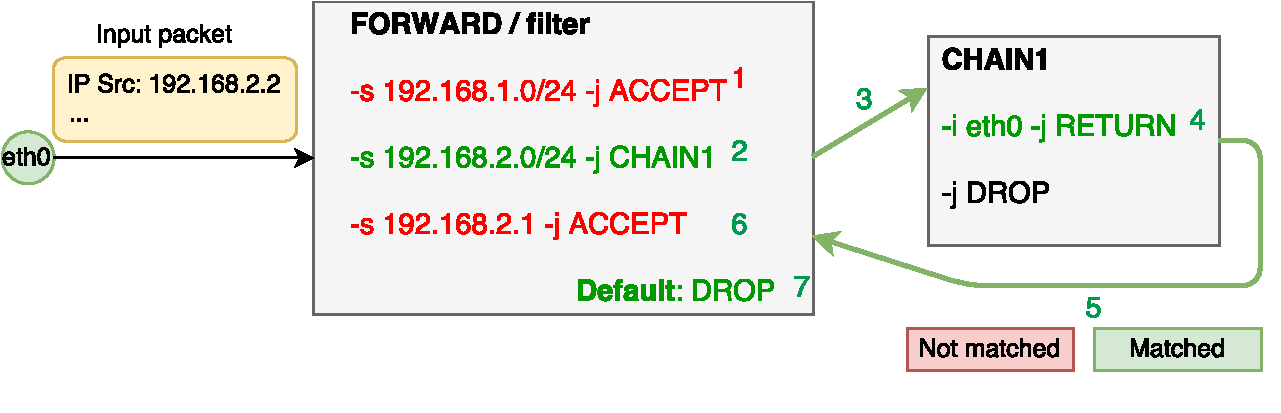
\includegraphics[scale=0.6]{assets/img/iptables-user-chains}
  \caption[Control flow of user-defined chains in iptables.]{Control flow of
  user-defined chains in iptables, featuring the \RETURN target.  Following the
  function analogy, \texttt{CHAIN1} here can be interpreted as a function that
  encapsulates the logic for filtering out traffic arrived on input interfaces
  other than \emph{eth0}.}
  \label{fig:iptables-user-chains}
\end{figure}

In order to include this behaviour in our chain SEFL models (i.e. chain IVDs),
let us first notice that as long as there is no rule in a chain that might jump
to a user-specified one, \labelindexref{Algorithm}{algo:chain-traversal} is
correct.  Thus, driven by the motivation to reduce our more complicated problem
to one that we know how to solve, we observe that we could obtain \RETURN-free
lists of rules by splitting our original one on boundaries given by rules that
might jump to user-defined chains (called hereafter \textbf{boundary rules}).

An (abstract) example of this idea is presented in
\labelindexref{Figure}{fig:splitting-rules}.  Rectangles correspond to rules in
a chain.  The ones that might jump to user chains are highlighted in red.
Following the boundary rule-splitting idea, three new ordered sublists of rules
result, as pointed out by the dashed brackets.

\begin{figure}[h]
  \centering
  \captionsetup{justification=centering}
  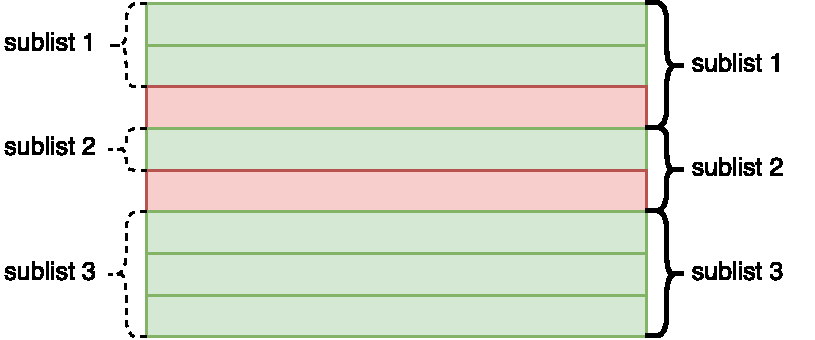
\includegraphics[scale=0.6]{assets/img/splitting-rules}
  \caption[Splitting rules in a chain on boundary rules.]{Splitting rules in a
  chain on boundary rules.  A boundary rule is a rule that might jump to a
  user-defined chain.}
  \label{fig:splitting-rules}
\end{figure}

How do we model this new internal structure of a chain IVD using SEFL?
Firstly, by decomposing its previously unified logic into multiple smaller IVDs
called \textbf{contiguous IVDs}. Each one of these new virtual devices that are
part of up a chain IVD implements the simple traversal algorithm presented in
the previous section for a sublist of rules.  Furthermore, to do this, it turns
out that we do not need to separate boundary rules from the sublist that
\textbf{precede} them.  This is indicated via bold brackets
\labelindexref{Figure}{fig:splitting-rules}.  This separation is not needed
because our splitting guarantees that the last rule in the previous sublist
does not jump to a user chain, and, thus, can lead to two actions only:
\begin{enumerate*}[a)]
  \item matching the rule and jumping to a built-in target (e.g. \texttt{NAT,
    ACCEPT, RETURN, MARK}), and
  \item not matching the rule and \emph{continuing} to the next one,
\end{enumerate*}
none of which could lead to a \RETURN to the succeeding one.  In other words,
we split only \textbf{after} boundary rules because that is the point we might
\textbf{need to return} to.

Besides organizing rules on contiguous IVDs, we also need to link them
together, such that if no rule matches in a contiguous IVD, packets are
forwarded to the next one.  Finally, we need to dispatch as part of our SEFL
model both input and returned packets, as follows:
\begin{itemize}
  \item \textbf{Input} packets to one of the (possibly) many contiguous IVDs
    that are part of a chain IVD.  That is, newly arrived packets should always
    be forwarded to the first one, while \emph{returning} packets should be
    forwarded to the one that follows the \emph{caller} IVD (using the function
    analogy from a previous paragraph).  To do this, a metadata field is
    allocated and assigned when performing jumps, and deallocated when
    returning.  This is essentially a SEFL stack.  The input dispatch is
    performed by a new virtual device component called
    \textbf{InputTagDispatcher}.
  \item \textbf{Returned} packets to the caller IVD. Since this is a dynamic
    decision too (i.e. multiple chains could jump to the same user chain),
    another tag is stored as a flow metadata which determines the
    \textbf{backlink} to forward the packet to.  The virtual device that does
    this is called \textbf{OutputTagDispatcher}.
\end{itemize}

The resulting internal organization of a virtual device that models a chain is
shown in \labelindexref{Figure}{fig:chain-internal}.

\begin{figure}[h]
  \centering
  \captionsetup{justification=centering}
  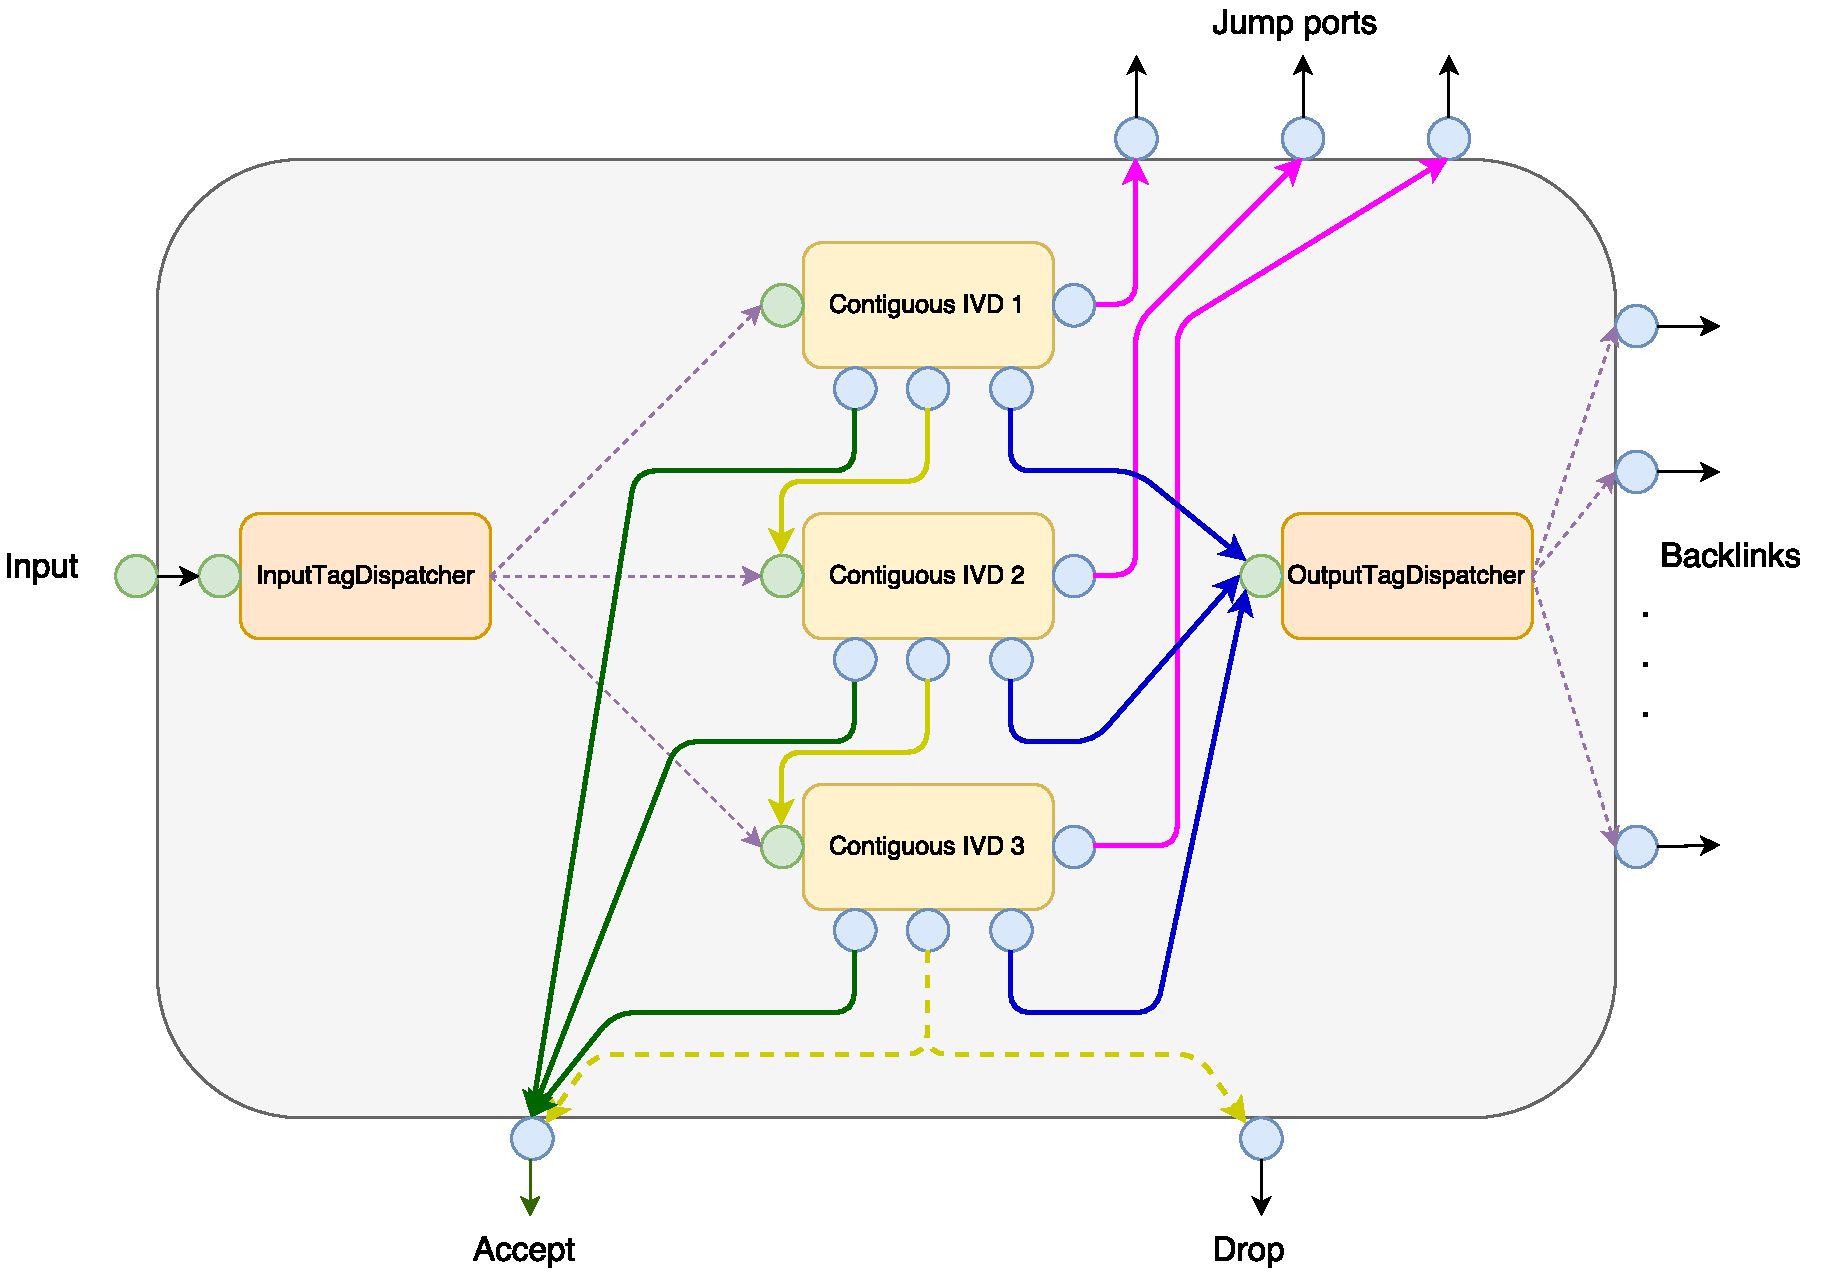
\includegraphics[scale=0.5]{assets/img/chain-internal}
  \caption[Internal organization of a chain IVD.]{Internal organization of a
  chain IVD.  It has one input port, one accept port, one drop port, a number
  of jump ports equal to the number of rules that might jump to user chains,
  and a variable (but still static) number of backlinks, that corresponds to
  the chains that might jump to this one.  Each \textbf{contiguous IVD} has 1
  input and 5 outputs: one for \texttt{ACCEPT} (green), one for \texttt{DROP}
  (skipped due to lack of space), one for forwarding packets to the next
  contiguous IVD (yellow; for the last one it is given by the chain policy),
  one for jumping to a user chain (magenta; only in the last rule of that
  sublist of rules), and, finally, one for returning to the caller chain (blue;
  managed by \textbf{OutputTagDispatcher}).}
  \label{fig:chain-internal}
\end{figure}

\bigskip

To summarize this section, we started with a model suitable for iptables
configurations that do not make use of the \RETURN target (and, thus, make
little use of user-defined chains) and have extended it to support the control
flow it adds.  We showed how we split a chain of rules into multiple sublists
that can then be modelled as separate contiguous IVDs, a new virtual device we
introduced that applies the naive algorithm presented in the previous section
(\labelindexref{Algorithm}{algo:chain-traversal}).  Finally, we illustrated how
all these new features play out together in a comprehensive diagram
(\labelindexref{Section}{fig:chain-internal}).


\section{The \emph{nat} table}

As mentioned at the beginning of this chapter, our goal is to add an increasing
number of features to an iptables-enabled device and see how they influence the
model we devised so far.  In this section we show why the \textbf{nat} table
needs special handling and adapt our model to it.

Network Address Translation (NAT) is a generic way of referring to one of the
many types of address translation that have been conceived over time.  In
addition to them, iptables introduces its own terminology including the
following important features (also listed in
\labelindexref{Appendix}{app:iptables-extensions}):
\begin{itemize}
  \item \SNAT : rewrites source IP/port with other IP/port (possibly from a
    given range); alternative names for this technique include
    \emph{many-to-one NAT}, \emph{port address translation}, \emph{NAT
    overload}.
  \item \DNAT : similar to the previous one but applied to destination IP/port;
    its most common use-case is \emph{port forwarding}.
  \item \REDIRECT : redirects packets to the machine itself; it is similar to
    \DNAT-ing to one of this machine's IP addresses.
  \item \MASQUERADE : this is the true \emph{many-to-one NAT} technique; in
    addition to the capabilities provided by regular \SNAT, it is resilient to
    interface-level changes (reset, IP change, etc).
\end{itemize}

In the given context, what does our current model fail to capture?  It is true
that all targets listed above have a well-defined effect on the flow they are
applied to, as shown in an example in
\labelindexref{Chapter}{chapter:background}
(\labelindexref{Figure}{fig:snat-example}).  It turns out that the problem is
not related to a specific target, but instead it has to do with the semantics
of the entire table as a whole, as the name of this section suggests.  To be
more precise, the following should be ensured:
\begin{itemize}
  \item Each chain in this table (i.e. PREROUTING, POSTROUTING and OUTPUT) is
    traversed \textbf{one time only} for each \emph{flow}.  The \emph{decision}
    (i.e.  target) taken is then automatically applied for each packet
    belonging to that flow.
  \item The \textbf{reverse translation} should be performed on \emph{reply}
    packets automatically.
\end{itemize}

To be more explicit, \labelindexref{Listing}{lst:nat-reply-sefl} shows how the
latter can be achieved in SEFL for a \SNAT-ed packet.  It is a simplified
version as it assumes TCP traffic only; to conform to the real implementation,
an additional \hltexttt{If} statement must be included to check that the L4
protocol is TCP.

\begin{minipage}{.6\textwidth}
\begin{listing}[H]
  \sourcecode{scala}{assets/code/nat-reply-sefl.scala}
  \caption{Sample SEFL code showing how reply packets are automatically
  rewritten in NAT-ed TCP connections.}
  \label{lst:nat-reply-sefl}
\end{listing}
\end{minipage}\hfill
\begin{minipage}{.36\textwidth}
  \centering
  % \captionsetup{justification=centering}
  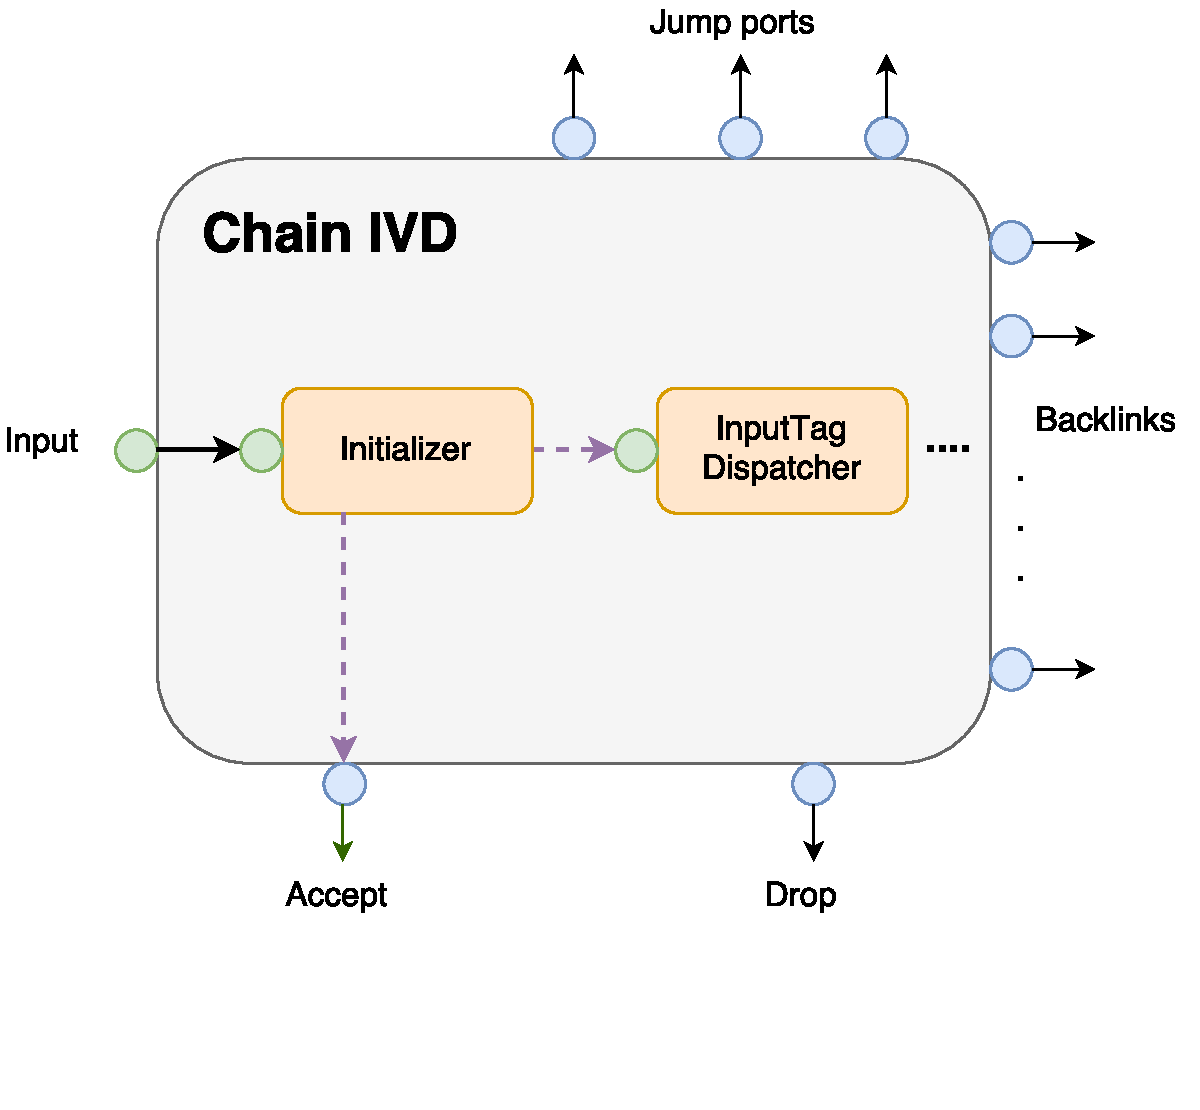
\includegraphics[scale=0.3]{assets/img/chain-internal-initializer}
  \captionof{figure}[Updated chain IVD model to accomodate the Initializer
  component.]{Updated chain IVD model to accomodate the Initializer component.}
  \label{fig:chain-internal-initializer}
\end{minipage}

\bigskip

The logic for automatically reapplying previous decisions is similar.  The only
question that remains is how do we \textbf{skip} the \emph{nat} table for these
connections?  In order to do so, we need to ensure that the corresponding SEFL
code is executed prior to dispatching packets to one of the contiguous IVDs,
which takes place in the InputTagDispatcher, as shown in
\labelindexref{Figure}{fig:chain-internal}.

Therefore, we introduce a new \emph{virtual device} that sits in front of the
InputTagDispatcher that can rewrite packets either as a reapplication of a
previous \emph{nat} decision, or as part of reply packets, and skip the whole
internal logic for the former.  It is called \textbf{Initializer}.
\labelindexref{Figure}{fig:chain-internal-initializer} shows how our previous
model of a chain IVD changes to include it.  Note that this new virtual device
is only really needed for chains which are part of the \emph{nat} table.


\section{Connection tracking}\label{sec:model-conntrack}

In \labelindexref{Section}{sub-sec:conntrack} of the previous chapter we
discussed the relation between iptables/netfilter and \textbf{conntrack}.  We
saw that while its business is kept separately from the other netfilter
components, it is embedded in the processing stack after the \emph{raw} table
in the PREROUTING and OUTPUT chains.

We also described the four states a connection can be in (\NEW, \ESTABLISHED,
\RELATED, \INVALID), as well as three additional virtual states that are used
in iptables rules (\UNTRACKED, \SNAT, \DNAT).  However, we did not mention how
to model the logic behind conntrack that controls the state of connections
associated with incoming packets.  In fact, there are certain limitations due
to our flow modelling based on SEFL that makes us unable to model some of them
(further discussed in \labelindexref{Section}{sec:limitations}).

What we do model are the transition to \NEW and the one between states \NEW and
\ESTABLISHED.  The former is as simple as marking flows as \NEW when the
metadata field that keeps track of the connection state is not set.  The latter
is analogous: we mark flows as \ESTABLISHED when a \emph{reply} packet that
belongs to a \NEW-tagged connection is received.

To augment the model we devised so far with this new tiny, but important logic,
we introduce a new \emph{virtual element} right after the chain IVDs
corresponding to the \emph{raw} table in the PREROUTING and OUTPUT chains.  The
result is shown in \labelindexref{Figure}{fig:conntrack-chain}.

\begin{figure}[h]
  \centering
  \captionsetup{justification=centering}
  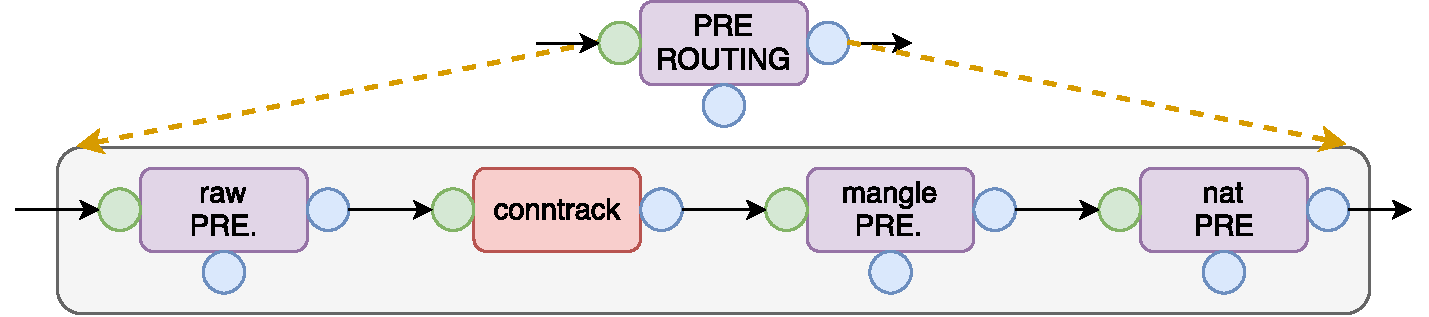
\includegraphics[scale=0.5]{assets/img/conntrack-chain}
  \caption[Element modelling conntrack transitions in the processing
  stack.]{Element modelling conntrack transitions in the processing stack.  The
  OUTPUT chain is analogous.}
  \label{fig:conntrack-chain}
\end{figure}


\section{Limitations}\label{sec:limitations}
Our model is built to mimic the netfilter implementation when stripping it to
the bare minimum that deals with packet flows.  This should be of no surprise
as it is one of the core design principles behind SEFL and SymNet: focus
only on execution paths in the original code that are tied to at least one
flow, and ignore boundary cases (i.e. out-of-memory errors, memory corruption,
etc).

This also means that we inherit all the modelling limitations of our toolset.
The most important ones have already been touched upon in
\labelindexref{Section}{sec:symnet-sefl}.  In the following paragraphs we
analyze the way these limitations reflect on our iptables model.

\paragraph{Global NAT state.}
One of the assumptions that SymNet makes as a consequence of having each
execution path tied to a packet flow is that global state is not captured.

One of the network function that makes use of global state is Network Address
Translation.  Besides the per-flow state, one thing that NAT network appliances
ensure is that there are no rewrite clashes across different connections.  For
instance, for a rule such as \hltexttt{-s 10.0.0.0/8 -j SNAT --to-source
1.1.1.1}, a NAT device guarantees that each source address belonging to the
specified network gets a different port number.  More than that, it can start
rejecting upstream traffic once the total number of simultaneous connections is
reached.  Note that this might happen due to a threshold imposed by the device
rather than consuming the entire port range (implicit in this rule).

However, that is a boundary case, not a rule that a network administrator would
be able to enforce nor want to.  In other words, if host \textbf{A} cannot
connect to server \textbf{B} because there are no ports available anymore, that
is a faulty situation which cannot be deterministically relied on.  Thus, the
benefit from modelling this behaviour would be negligible even if we were able
to.

\begin{figure}[h]
  \centering
  \captionsetup{justification=centering}
  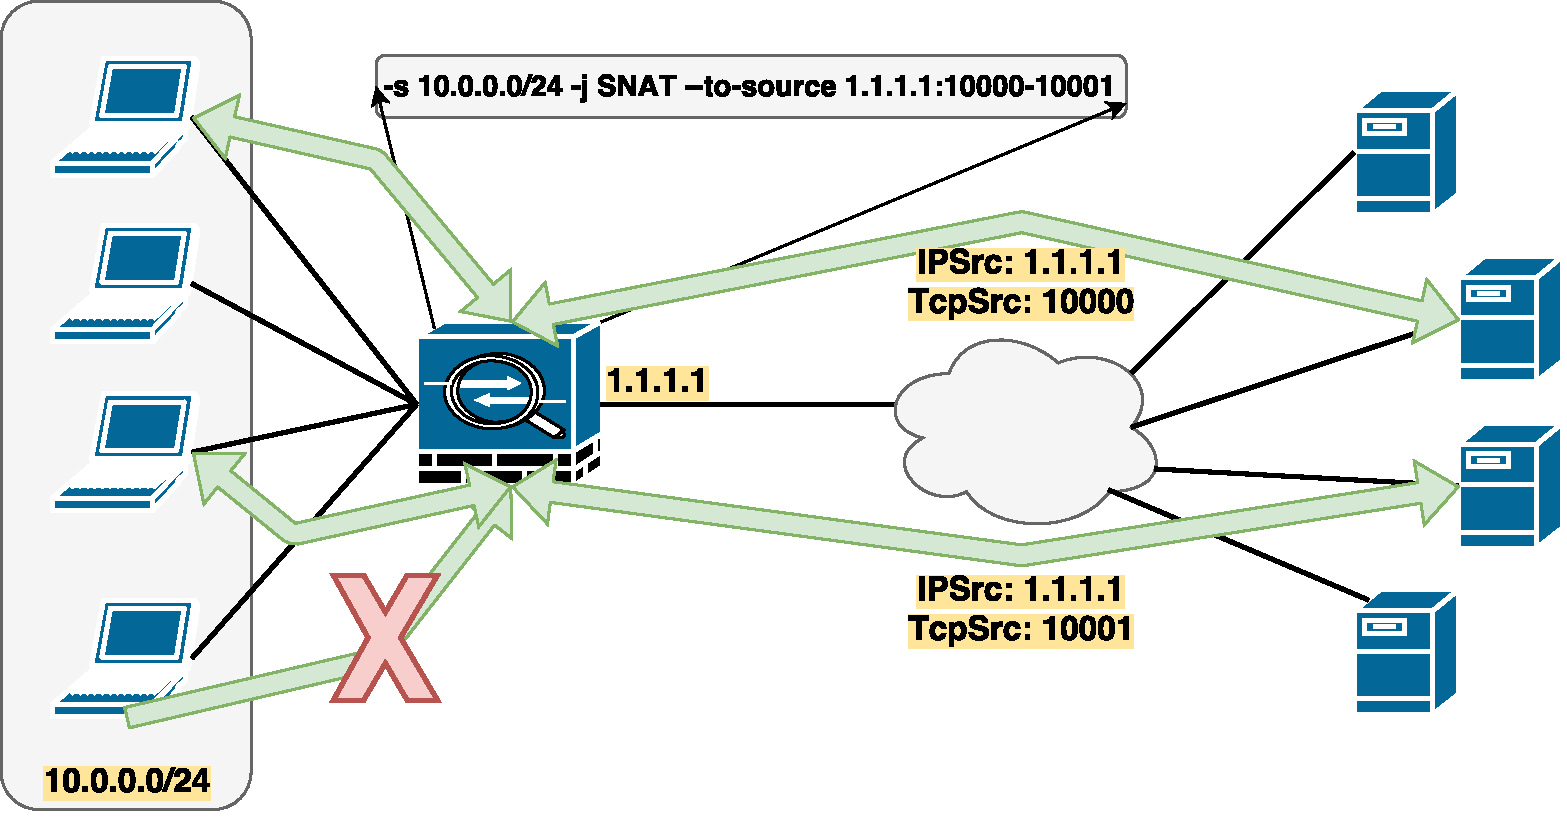
\includegraphics[scale=0.5]{assets/img/nat-global-state}
  \caption[Connection is rejected by NAT appliance due to no available ports
  remaining.]{Connection is rejected by NAT appliance due to no available ports
  remaining. The SNAT rule gives a range with only two ports which makes the
  third connection initiation to be rejected by the NAT box.  This can only be
  accomplished by keeping track of state across flows.}
  \label{fig:nat-global-state}
\end{figure}

\paragraph{\RELATED (connection state).}
In \labelindexref{Section}{sec:model-conntrack} we left unmodelled some of the
states a connection can be.  In particular, the \RELATED state is one which
comes up often in iptables rules.  Informally, a connection is considered
\RELATED when it is \textbf{caused} by another established one.  This includes
all \emph{data connections} which are started as part of a protocol that have a
dedicated \emph{control connection}.

The reason it cannot be modelled stems from the \textbf{flows independence}
design assumption: the two connections correspond to two different flows which
simply cannot be \emph{related} by our network description language.

\begin{figure}[h]
  \centering
  \captionsetup{justification=centering}
  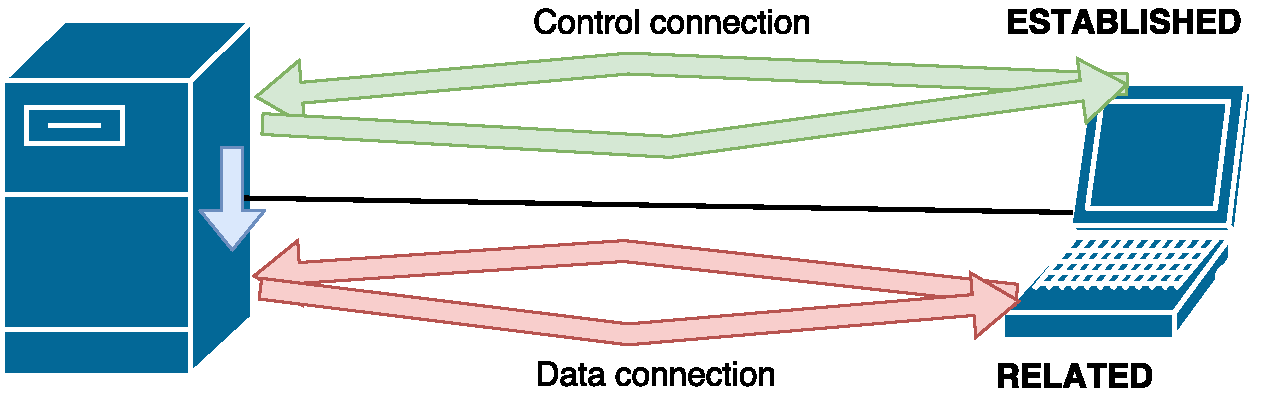
\includegraphics[scale=0.5]{assets/img/related-state}
  \caption{A control (established) connection starts a new data (related)
  connection.}
  \label{fig:related-state}
\end{figure}

\paragraph{Local process.}
In the block diagrams showing the internal components of our iptables model
(\labelindexref{Figure}{fig:iptables-2}) we included one that abstracts the
local process.  This was done to be on par with the internal organization of
iptables featured in the previous chapter
(\labelindexref{Figure}{fig:iptables-organization}).

A very accurate model of the local process would be the source code itself,
which would imply running symbolic execution on the entire kernel and the
applications that sit on top of it.  This is obviously intractable.

An alternative inspired by how entire networks are modelled with SEFL is to
focus only on simplified application-specific behaviours.  In fact, our design
allows embedding such user-specified custom logic.  For instance, a very raw
model of a server would only swap source and destination addresses and forward
the packet to the OUTPUT chain.  Alternatively, the simplest local process
would act as a \emph{sink}, not doing anything with incoming packets which
causes symbolic execution to consider that flow a success.

Additionally, a design choice we made to allow bootstrapping symbolic execution
with traffic originating from an iptables-enabled device is to \textbf{expose}
the output port of the \emph{virtual device} that abstracts the local process
(\labelindexref{Figure}{fig:local-process-out}).  This is an alternative,
simplified way of modelling certain applications, as shown above, but only for
outbound traffic.

\begin{figure}[h]
  \centering
  \captionsetup{justification=centering}
  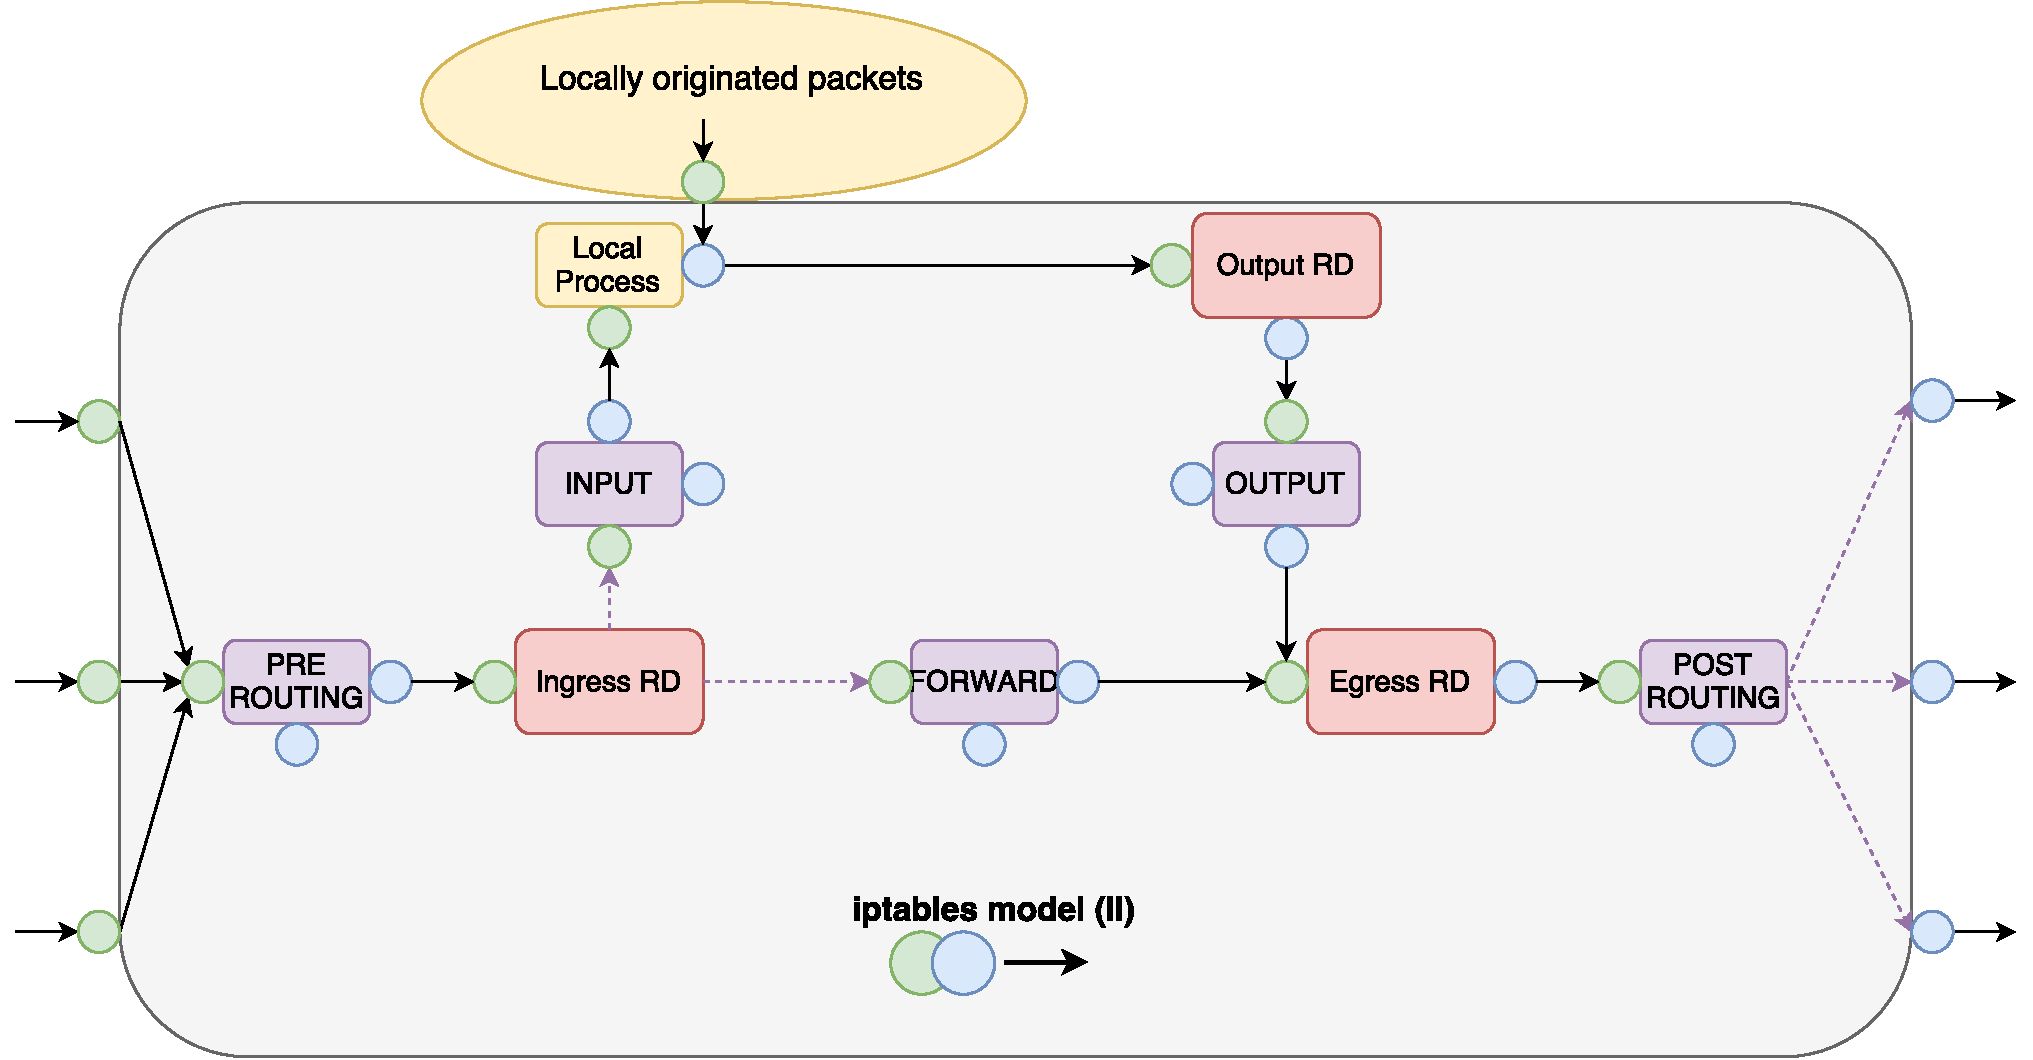
\includegraphics[scale=0.4]{assets/img/local-process-out}
  \caption[Exposing the output port of the local process VD.]{Exposing the
  output port of the local process VD to allow injecting packets on it, and,
  thus, simulating locally originated traffic.}
  \label{fig:local-process-out}
\end{figure}


\section{Summary}
In this chapter we derived a model for an iptables-enabled device starting from
a simple router.

We started by building a processing stack in which each chain is modelled as a
separate entity that encapsulates the traversal of a list of rules.  We
continued by adding support for user-defined chains and the \RETURN target.
Together, they introduce a new traversal order that resembles function calls in
procedural languages.  Next, we dedicated two sections to show that the
\emph{nat} table and \emph{connection tracking} need dedicated logic.  Once we
solved (some of) the issues they introduced, we can finally assert that the
resulting model is the final one.  We followed that up with a discussion about
its limitations.

In the next two chapters we present the internal design and implementation
choices behind the \TOOL tool, and evaluate the models we construct from
various iptables configurations.
